% L5a lecture companion: follow the approved notebook's teaching order.
% Setup remains in the notebook, as in the L4a deck convention.
% Standalone TikZ diagrams and per-figure Makefiles live in ../figs/.
\documentclass[aspectratio=169,11pt]{beamer}
\usepackage{vnslides}
\usepackage{tabularx}

\renewcommand{\vnlecturecode}{L5a}
\newcolumntype{Y}{>{\raggedright\arraybackslash}X}
\newcommand{\lecturelink}{https://github.com/varnerlab/CHEME-5800-CourseRepository-Fall-2026/blob/main/weeks/week-05/L5a/CHEME-5800-L5a-Lecture-MaximumFlowProblems-Fall-2026.ipynb}
\newcommand{\examplelink}{https://github.com/varnerlab/CHEME-5800-CourseRepository-Fall-2026/blob/main/weeks/week-05/L5a/CHEME-5800-L5a-WorkedExample-MaximumFlow-Fall-2026.ipynb}
\newcommand{\lablink}{https://github.com/varnerlab/CHEME-5800-CourseRepository-Fall-2026/blob/main/weeks/week-05/L5b/CHEME-5800-L5b-Lab-MaximumFlowSensitivity-Fall-2026.ipynb}

\title{\texorpdfstring{{\vnheavy L5a}}{L5a}: Network-Flow Models}
\subtitle{\texorpdfstring{Capacity, conservation, and maximum flow\\[3pt]CHEME 5800 Cornell University}{Capacity, conservation, and maximum flow; CHEME 5800 Cornell University}}
\author{Copyright Jeffrey Varner 2026. All Rights Reserved}

\begin{document}
\special{pdf:minorversion 7}

\vntitlepage

% Notebook: introduction and learning objectives.
\begin{frame}{Objectives for Today}
  How much flow can a capacity-limited network deliver, and how can we show
  that this amount is the maximum?

  \vspace{0.8em}
  {\large\textbf{\ink{Today's concepts}}}
  \vspace{0.35em}
  \begin{itemize}\setlength{\itemsep}{0.7em}
    \item \hilite{Formulate the problem}: define capacities, conservation,
      and net source outflow.
    \item \hilite{Apply Ford–Fulkerson}: construct residual graphs, revise
      earlier routes, and choose augmenting paths.
    \item \hilite{Verify maximum flow}: check feasibility and use an upper
      bound from edge capacities to prove that more flow is impossible.
  \end{itemize}

  \slidenote{Lecture:}{\href{\lecturelink}{Network-flow models: capacity, conservation, and maximum flow}}
\end{frame}

% Notebook: Examples. Computational setup stays in the linked notebooks.
\begin{frame}{Lecture and Example}
  \textbf{\ink{Lecture:}}
  \href{\lecturelink}{Network-flow models}

  Formulate a flow problem, increase flow through residual paths, and
  establish a bound on what the network can deliver.

  \vspace{1.2em}
  \textbf{\ink{Example:}}
  \href{\examplelink}{Maximum flow in a worker–task network}

  How many assignments can the workers complete? Build the network, compute
  flows using two path-search rules, and check the results.

  \vspace{0.8em}
  One unit of flow represents \hilite{one completed assignment}.
\end{frame}

% Notebook: Formulating a maximum-flow problem.
\begin{frame}{Formulating a Maximum-Flow Problem}
  Represent the application as a finite directed graph
  $\mathcal G=(\mathcal V,\mathcal E)$ with vertices $\mathcal V$ and edges
  $\mathcal E$.

  \vspace{0.7em}
  \begin{itemize}\setlength{\itemsep}{0.7em}
    \item The \hilite{source} $s$ supplies flow; the \hilite{sink} $t$ receives
      it, with $s\ne t$.
    \item Each original edge $(u,v)$ has a finite \hilite{capacity}
      $c(u,v)\geq0$.
    \item The \hilite{flow} $f(u,v)$ is the amount assigned to that edge,
      in the same units as the capacity.
  \end{itemize}

  \vspace{0.5em}
  Worker availability and task limits become capacities. Data transmission
  and material transport use the same formulation.
\end{frame}

\begin{frame}{Capacity and Conservation Define Feasibility}
  Each original edge's flow $f(u,v)$ must stay within its capacity $c(u,v)$:
  \[
    \underbrace{0\leq f(u,v)\leq c(u,v)}_{\text{capacity constraint}},
    \qquad (u,v)\in\mathcal E.
  \]

  At an intermediate vertex $v\in\mathcal V\setminus\{s,t\}$, incoming
  and outgoing flow must balance:
  \[
    \underbrace{\sum_{u:(u,v)\in\mathcal E}f(u,v)}_{\text{inflow}}
    =\underbrace{\sum_{w:(v,w)\in\mathcal E}f(v,w)}_{\text{outflow}}.
  \]

  Intermediate vertices neither create nor consume flow. A
  \hilite{feasible flow} satisfies both constraints.
\end{frame}

\begin{frame}{Maximize Net Flow Leaving the Source}
  The flow value $|f|$ measures net outflow from the source $s$:
  \[
    |f|=
    \underbrace{\sum_{v:(s,v)\in\mathcal E}f(s,v)}_{\text{leaving }s}
    -\underbrace{\sum_{u:(u,s)\in\mathcal E}f(u,s)}_{\text{entering }s}.
  \]
  The source and sink are exempt from conservation: the source creates flow
  and the sink consumes it. Conservation at the intermediate vertices makes
  $|f|$ equal to the net inflow at the sink $t$.

  \vspace{0.5em}
  The maximum-flow problem seeks a feasible flow $f^*$ with the largest value:
  \[
    |f^*|=\max_{f\;\text{feasible}}|f|.
  \]

  \slidenote{Equivalently:}{imagine an edge entering the source from outside the network and an edge leaving the sink to outside the network, each carrying $|f|$; then every vertex balances.}
\end{frame}

% Notebook: Ford-Fulkerson Method; What is a Residual Graph?
\begin{frame}{Ford–Fulkerson Method}
  Start with zero flow. Repeatedly find an \hilite{augmenting path}: a
  source-to-sink route along which we can still send more flow.

  \vspace{0.8em}
  A \hilite{residual graph} records where we can add flow and where we can
  take back flow assigned earlier:
  \begin{itemize}\setlength{\itemsep}{0.8em}
    \item \hilite{Forward edges} record unused capacity.
    \item \hilite{Backward edges} record flow we can cancel to revise an
      earlier routing choice.
  \end{itemize}

  \vspace{0.7em}
  Ford–Fulkerson is a \hilite{method}: it leaves the path-selection rule
  open, and different rules give different algorithms.
\end{frame}

\begin{frame}{What Is a Residual Graph?}
  Suppose the original edge $(u,v)$ has capacity $c(u,v)=5$ and currently
  carries flow $f(u,v)=3$.

  \vspace{0.9em}
  \begin{columns}[T,onlytextwidth]
    \begin{column}{0.47\textwidth}
      \textbf{\ink{Forward: add flow}}

      \vspace{0.4em}
      Unused capacity from $u$ to $v$:
      \[
        c(u,v)-f(u,v)=\hilite{2}.
      \]
    \end{column}
    \begin{column}{0.47\textwidth}
      \textbf{\ink{Backward: cancel flow}}

      \vspace{0.4em}
      Flow we can cancel using $v\to u$:
      \[
        f(u,v)=\hilite{3}.
      \]
    \end{column}
  \end{columns}

  \vspace{1.0em}
  A backward residual edge is bookkeeping. It reduces an existing flow;
  it does not require a physical reverse connection.
\end{frame}

\begin{frame}{Defining Residual Capacities}
  Assume no self-loops or oppositely directed pairs of original edges.
  For an ordered pair $(u,v)$, the residual capacity is:
  \[
    \texttt{residual}(u,v)=
    \begin{cases}
      c(u,v)-f(u,v), & (u,v)\in\mathcal E,\\
      f(v,u), & (v,u)\in\mathcal E,\\
      0, & \text{otherwise.}
    \end{cases}
  \]

  The residual graph $\mathcal G_f=(\mathcal V,\mathcal E_f)$ retains all
  vertices and includes only edges with positive residual capacity:
  \[
    \mathcal E_f=\{(u,v)\in\mathcal V\times\mathcal V:
      \texttt{residual}(u,v)>0\}.
  \]

  \slidenote{Backward edges:}{because $\mathcal E_f$ is built from all ordered pairs, $(v,u)$ appears whenever $f(u,v)>0$, even though $(v,u)$ is not an original edge.}
\end{frame}

% Notebook: How do we augment the flow?
\begin{frame}{How Do We Augment the Flow?}
  An \hilite{augmenting path} $P$ is a directed path from $s$ to $t$ in the
  residual graph. Every edge on it has positive residual capacity.

  \vspace{0.7em}
  The largest increase $\Delta$ along the chosen path is its
  \hilite{bottleneck capacity}:
  \[
    \Delta=\min_{(u,v)\in P}\texttt{residual}(u,v).
  \]

  \begin{itemize}\setlength{\itemsep}{0.8em}
    \item On a forward edge, $\Delta$ limits how much flow we can add.
    \item On a backward edge, $\Delta$ limits how much flow we can cancel.
  \end{itemize}

  \vspace{0.5em}
  Use the same $\Delta$ on every path edge to preserve conservation.
\end{frame}

\begin{frame}{A Reverse Edge Revises an Earlier Route}
  All five original edges have capacity one.

  \vspace{0.7em}
  \begin{columns}[T,onlytextwidth]
    \begin{column}{0.48\textwidth}
      \centering
      \textbf{\ink{First flow: $|f|=1$}}

      \vspace{0.4em}
      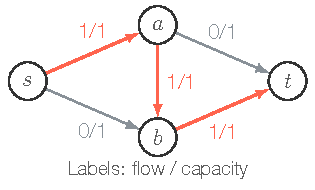
\includegraphics[width=\linewidth]{../figs/Fig-Residual-FirstFlow/Fig-Residual-FirstFlow.pdf}

      $s\to a\to b\to t$
    \end{column}
    \begin{column}{0.48\textwidth}
      \centering
      \textbf{\ink{Residual path: $\Delta=1$}}

      \vspace{0.4em}
      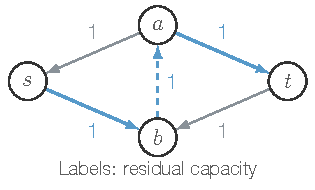
\includegraphics[width=\linewidth]{../figs/Fig-Residual-Augmentation/Fig-Residual-Augmentation.pdf}

      $s\to b\to a\to t$
    \end{column}
  \end{columns}

  \vspace{0.7em}
  The dashed step $b\to a$ cancels the earlier flow on $(a,b)$.
\end{frame}

\begin{frame}{Rerouting Raises the Flow Value to Two}
  Augment along $s\to b\to a\to t$ with $\Delta=1$.

  \vspace{0.8em}
  \begin{columns}[c,onlytextwidth]
    \begin{column}{0.46\textwidth}
      \centering
      \textbf{\ink{Revised flow: $|f|=2$}}

      \vspace{0.4em}
      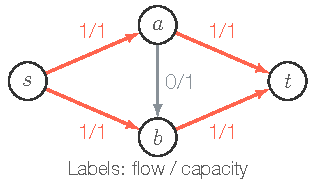
\includegraphics[width=\linewidth]{../figs/Fig-Residual-RevisedFlow/Fig-Residual-RevisedFlow.pdf}

      $s\to a\to t$ and $s\to b\to t$
    \end{column}
    \begin{column}{0.50\textwidth}
      \textbf{\ink{Original edge updates}}

      \vspace{0.5em}
      \renewcommand{\arraystretch}{1.3}
      \begin{tabular}{lll}
        \toprule
        Edge & Before & After\\
        \midrule
        $(s,b)$ & 0 & 1\\
        $(a,b)$ & 1 & 0\\
        $(a,t)$ & 0 & 1\\
        \bottomrule
      \end{tabular}

      \vspace{0.6em}
      Other edge flows stay at one; conservation is preserved.
    \end{column}
  \end{columns}

\end{frame}

\begin{frame}{Ford–Fulkerson Procedure}
  Initialize $f(u,v)=0$ for every original edge. Then repeat:

  \vspace{0.8em}
  \begin{enumerate}\setlength{\itemsep}{0.8em}
    \item Construct the residual graph and find a path $P$ from $s$ to $t$.
      If no path exists, stop.
    \item Find the bottleneck $\Delta$ along $P$.
    \item Add $\Delta$ to each forward edge's flow; subtract $\Delta$ from
      the original flow corresponding to each backward edge.
    \item Recompute residual capacities before searching again.
  \end{enumerate}

  \vspace{0.7em}
  Each augmentation preserves feasibility and increases $|f|$ by $\Delta$.
\end{frame}

% Notebook: How do we find augmenting paths? Edmonds–Karp, then the two rules compared.
\begin{frame}{Edmonds–Karp Uses Breadth-First Search}
  Search the residual graph using \hilite{breadth-first search}, following
  only edges with positive residual capacity.

  \vspace{0.6em}
  \begin{itemize}\setlength{\itemsep}{0.6em}
    \item Choose an augmenting path with the fewest edges.
    \item Neighbor order breaks ties between equal-length paths.
    \item Update residual capacities and search again after each augmentation.
  \end{itemize}

  \vspace{0.4em}
  With adjacency lists and exact arithmetic, the worst-case running time is:
  \[
    \mathcal O\!\left(|\mathcal V|\,|\mathcal E|^2\right).
  \]
  The bound depends on graph size, not capacity values.

  \slidenote{Reference:}{\href{https://algs4.cs.princeton.edu/64maxflow/}{Sedgewick and Wayne, Algorithms: Maximum Flow}}
  \note{[Sources]\newline https://algs4.cs.princeton.edu/64maxflow/\newline Edmonds–Karp running-time bound.\newline [/Sources]}
\end{frame}

\begin{frame}{Two Path-Selection Rules for the Same Method}
  The \href{\examplelink}{worker–task example} applies the Ford–Fulkerson
  method with two path-selection rules to the same capacities.

  \vspace{0.7em}
  \renewcommand{\arraystretch}{1.4}
  \begin{tabularx}{\textwidth}{YY}
    \toprule
    \textbf{Path-selection rule} & \textbf{Behavior}\\
    \midrule
    Depth-first search & Takes the first augmenting path it reaches; may choose longer paths\\
    Breadth-first search (Edmonds–Karp) & Chooses an augmenting path with the fewest edges\\
    \bottomrule
  \end{tabularx}

  \vspace{0.7em}
  Both searches give the same maximum-flow value. Their individual
  worker–task assignments may differ.

  \vspace{0.5em}
  With integer capacities, each augmentation adds at least one unit, so
  either search terminates.
\end{frame}

% Notebook: Verifying feasibility and maximum flow.
\begin{frame}{Verifying Feasibility and Maximum Flow}
  Ford–Fulkerson stops when no augmenting path remains. How do we know the
  returned flow is the largest possible, and not merely the largest this
  sequence of paths could find? First, check feasibility:

  \vspace{0.6em}
  \begin{enumerate}\setlength{\itemsep}{0.7em}
    \item \hilite{Capacities}: every original edge satisfies
      $0\leq f(u,v)\leq c(u,v)$.
    \item \hilite{Conservation}: each intermediate vertex has equal total
      inflow and outflow.
    \item \hilite{Source–sink balance}: net source outflow equals net sink
      inflow.
  \end{enumerate}

  \vspace{0.6em}
  These checks establish only that the flow is allowed. To prove it is
  maximum, we need an upper bound that the feasible flow reaches.
\end{frame}

\begin{frame}{A Source–Sink Cut Gives an Upper Bound}
  A \hilite{source–sink cut} partitions $\mathcal V$ into disjoint sets
  $S$ and $T$, with $s\in S$ and $t\in T$.

  \vspace{0.8em}
  \begin{columns}[c,onlytextwidth]
    \begin{column}{0.52\textwidth}
      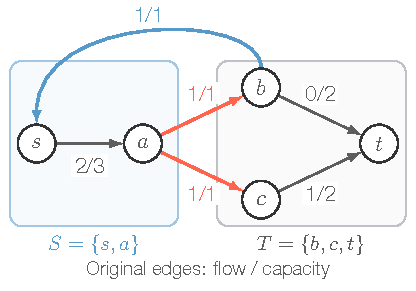
\includegraphics[width=\linewidth]{../figs/Fig-Cut-Balance/Fig-Cut-Balance.pdf}
    \end{column}
    \begin{column}{0.44\textwidth}
      The cut capacity is the sum of the original edge capacities from $S$ to $T$:
      \[
        c(S,T)=\sum_{\substack{(u,v)\in\mathcal E\\u\in S,\;v\in T}}c(u,v).
      \]
      The two \hilite{outgoing cut edges} give $c(S,T)=1+1=2$.

      \vspace{0.6em}
      The \textcolor{vnslidelink}{edge $b\to s$} is an original edge that
      enters the source. It crosses from $T$ to $S$ and adds no cut capacity.
    \end{column}
  \end{columns}
\end{frame}

\begin{frame}{Cut Balance Bounds Every Feasible Flow}
  Sum net outflows over vertices in $S$. Internal edge flows cancel, and
  conservation leaves only the source's net outflow:
  \[
    |f|=
    \underbrace{\sum_{\substack{(u,v)\in\mathcal E\\u\in S,\;v\in T}}f(u,v)}_{S\to T}
    -\underbrace{\sum_{\substack{(u,v)\in\mathcal E\\u\in T,\;v\in S}}f(u,v)}_{T\to S}.
  \]

  Forward flow is at most its capacity; return flow is nonnegative. Thus:
  \[
    |f|\leq
    \sum_{\substack{(u,v)\in\mathcal E\\u\in S,\;v\in T}}c(u,v)
    =c(S,T).
  \]

  Every source–sink cut therefore bounds every feasible flow.
\end{frame}

\begin{frame}{No Augmenting Path Identifies a Cut}
  When $t$ is unreachable, let $S$ contain the vertices reachable from $s$
  in the residual graph; $T=\mathcal V\setminus S$.

  \vspace{0.5em}
  \begin{columns}[c,onlytextwidth]
    \begin{column}{0.52\textwidth}
      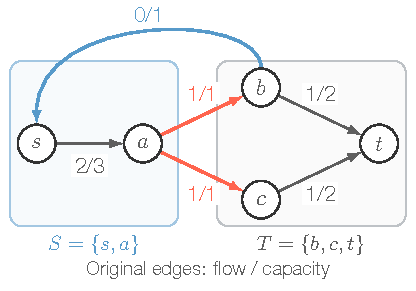
\includegraphics[width=\linewidth]{../figs/Fig-Cut-Optimality/Fig-Cut-Optimality.pdf}
    \end{column}
    \begin{column}{0.44\textwidth}
      \textbf{\hilite{$S\to T$: saturated}}

      Unused capacity would let the residual search enter $T$.

      \vspace{0.8em}
      \textbf{\textcolor{vnslidelink}{$T\to S$: zero flow}}

      Positive flow would create a backward residual edge into $T$.
    \end{column}
  \end{columns}

  \vspace{0.3em}
  $S\to T$ edges are full and the $T\to S$ edge is empty, so $|f|=c(S,T)=2$.
\end{frame}

\begin{frame}{The Stopping Condition Proves Maximum Flow}
  Substitute saturated $S\to T$ edges and zero $T\to S$ flows into the
  cut balance:
  \[
    |f|=c(S,T).
  \]
  The feasible flow reaches a bound on every feasible flow. It is therefore
  maximum, and the cut has minimum capacity.

  \vspace{0.6em}
  The \hilite{maximum-flow/minimum-cut theorem} states:
  \[
    \max_{f\;\text{feasible}}|f|
    =\min_{(S,T)\;\text{source–sink cut}}c(S,T).
  \]

  \slidenote{Reference:}{\href{https://courses.csail.mit.edu/6.854/21/Notes/n06-flow.html}{David Karger, MIT 6.854: Flow}}
  \note{[Sources]\newline https://courses.csail.mit.edu/6.854/21/Notes/n06-flow.html\newline Cut bound and maximum-flow/minimum-cut theorem.\newline [/Sources]}
\end{frame}

\begin{frame}{Three Assignments Reach the Source-Cut Bound}
  The default worker–task network has three source-to-worker edges,
  each with capacity one assignment.

  \vspace{0.7em}
  \begin{columns}[c,onlytextwidth]
    \begin{column}{0.47\textwidth}
      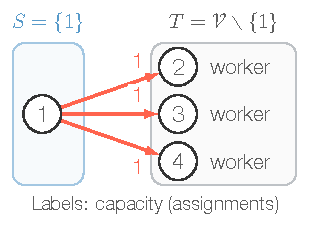
\includegraphics[width=\linewidth]{../figs/Fig-Worker-SourceCut/Fig-Worker-SourceCut.pdf}
    \end{column}
    \begin{column}{0.49\textwidth}
      Put the source, node 1, in $S$ and every other vertex in $T$. The cut capacity is:
      \[
        c(S,T)=1+1+1=\hilite{3}.
      \]
      The \href{\examplelink}{worked example} attains this bound:
      \[
        |f|=c(S,T)=3.
      \]
      Therefore, the maximum is \hilite{three assignments}. Each worker
      can take one assignment, so the fourth task goes unassigned.
    \end{column}
  \end{columns}

  \slidenote{Next:}{\href{\lablink}{L5b changes capacities} and examines how the maximum number of assignments changes.}
\end{frame}

% Notebook: Summary, with three retrospective takeaways and the L5b connection.
\begin{frame}{Summary}
  We formulated, computed, and verified maximum flow.

  \vspace{0.6em}
  {\large\textbf{\ink{Key takeaways}}}
  \vspace{0.3em}
  \begin{itemize}\setlength{\itemsep}{0.6em}
    \item \textbf{\ink{Capacity and conservation.}} We maximized net source
      outflow subject to edge capacities and intermediate flow balances.
    \item \textbf{\ink{Residual augmentation.}} We used bottlenecks to add
      or cancel flow while preserving feasibility, and compared depth-first
      search with Edmonds–Karp, which chooses paths with the fewest edges.
    \item \textbf{\ink{Proof of maximum flow.}} We matched feasible flow
      to a cut bound, proving a maximum of three assignments in our example.
  \end{itemize}

  \vspace{0.5em}
  In \href{\lablink}{L5b}, we examine how capacity changes affect this maximum.
\end{frame}

\end{document}
